% analysis.tex
%

%% ==============
\chapter{Comissioning measurements and analysis}
\label{ch:Analysis}
%% ==============

  While the moun detection system was still under construction at the beginning of my thesis-work, first measurements were taken at the time with some modules under preliminary conditions to look into the behaviour of these modules. Step by step, the system was completed and is now up and running. In the building phase, several measurements and test have been conducted to ensure the capabilities of the system meet the requirements for the KATRIN experiment. Starting with the setup of acceleration voltages, gains and thresholds, 
  Using data obtained by the muon modules and the detector as well as other subsystems' data, the muon induced background rates and both spatial and energy distribution can be obtained. Before actual measurements were done, the modules had to be set up and calibrated, meaning high voltage and signal cabling needed to be installed and high voltage power supplies had to be acquired.
   
  
  
  
  %% ===========================
  \section{Finding the best filter settings}
  \label{ch:Analysis:sec:Finding the best filter settings}
  %% ===========================  
 
  
  As the PMT tubes are directly, without any preamplifiers, connected to the DAQ, the signal lengths arriving at the latter are in the order of \SI{20}{\nano\second}. This poses a problem for filters as the sampling rates need to be high and anti-aliasing is inevitable. To find the best settings, a function generator has been set up to create events at known frequency and peak heigth. The pulser's signal form \todo{what form} was chosen as closely to the actual shape as possible, which is the "pin diode" form.
 
  \begin{figure}
	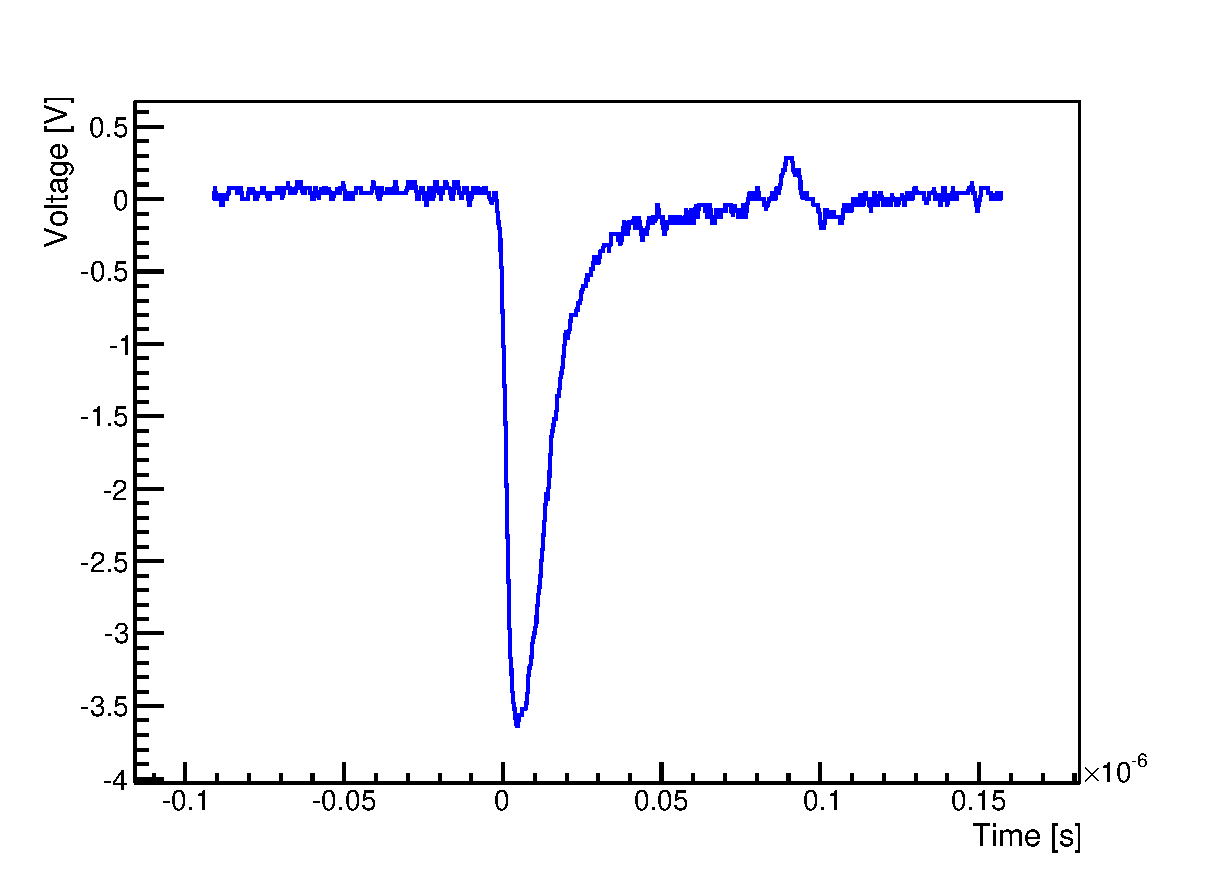
\includegraphics[width = 0.9\textwidth]{graphics/muonModules/monSpec/muonSignal.eps}
	\caption[Muon signal shape]{Pulser shape on the left compared to actual signal shape on the right. }
  \end{figure}
	\begin{figure}
	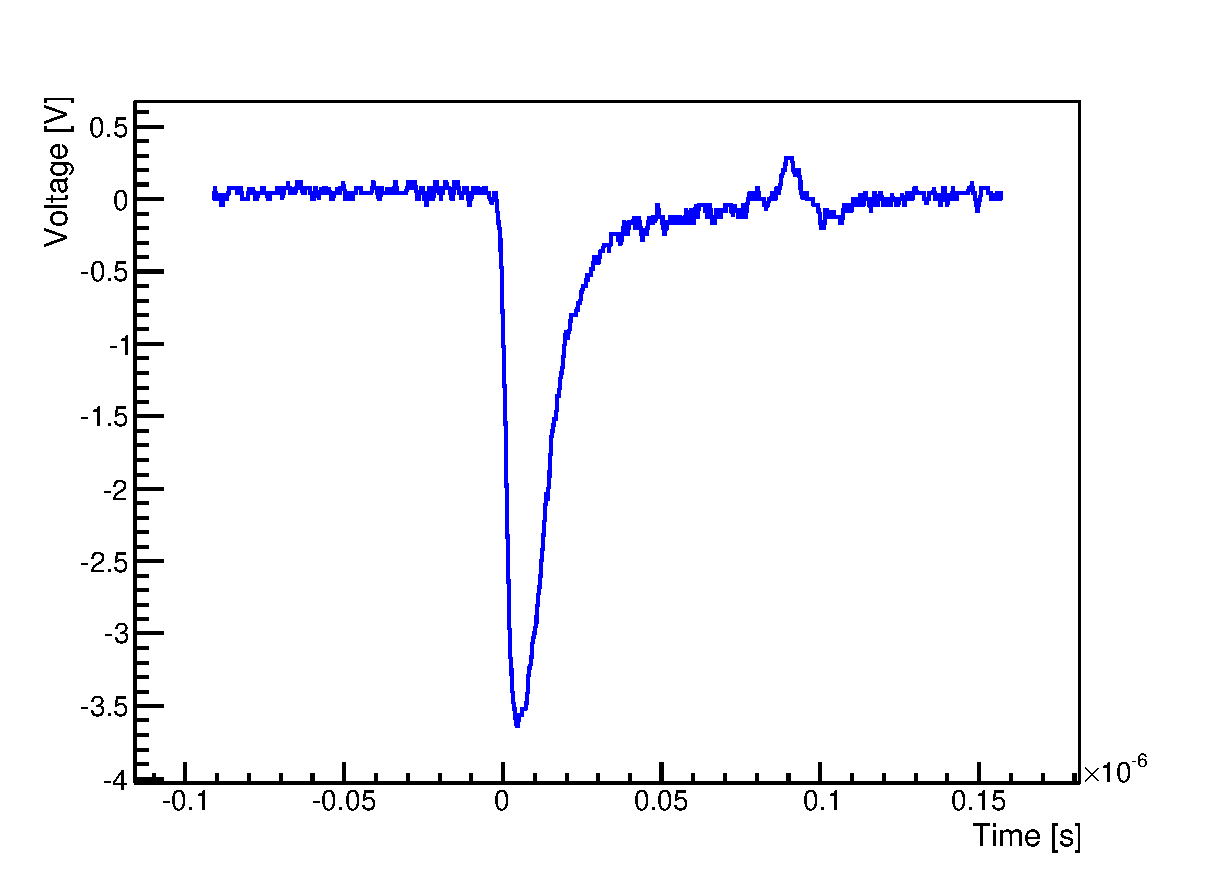
\includegraphics[width = 0.9\textwidth]{graphics/muonModules/monSpec/muonSignal.eps}
	\caption[Pulser and signal shape]{Pulser shape on the left compared to actual signal shape on the right. }
  \end{figure}
  
  In order to evaluate filter's figure of merit, the width of the resulting energy histogram, which should, assuming perfect pulser signals and perfect filters, be mono-energetic, was analyzed for each filter setting. For analysis, the width of the contributing ADC bins and their absolute position as well as the pulse height and the filter settings were noted. 
  
  \begin{table}
	\centering
  	\begin{tabular}{|c|c|c|c|c|}
  		\hline
  		Voltage[V] & Boxcar length [ns] & width & position & threshold\\
  		\hline
  		\multirow{4}{*}{1} & 50 & 33 & 2160 & 2100\\
  		 & 100 & 37 & 2140 & 4200\\
  		 & 150 & 13 & 2140 & 6300\\
  		 & 200 & 21 & 2141 & 8400\\
  		 \hline
  		 \multirow{4}{*}{2} & 40 & 25 & 2160 & 2100\\
  		 & 100 & 78 & 2140 & 4200\\
  		 & 150 & 78 & 2140 & 6300\\
  		 & 200 & 77 & 2141 & 8400\\
  		 \hline
  		 \multirow{4}{*}{3} & 59 & 25 & 2160 & 2100\\
  		 & 100 & 113 & 2140 & 4200\\
  		 & 150 & 110 & 2140 & 6300\\
  		 & 200 & 112 & 2141 & 8400\\
  		 \hline
  		 \multirow{4}{*}{4} & 80 & 25 & 2160 & 2100\\
  		 & 100 & 145 & 2140 & 4200\\
  		 & 150 & 147 & 2140 & 6300\\
  		 & 200 & 149 & 2141 & 8400\\
  		 \hline
  		 \multirow{4}{*}{5} & 94 & 25 & 2160 & 2100\\
  		 & 100 & 180 & 2140 & 4200\\
  		 & 150 & 185 & 2140 & 6300\\
  		 & 200 & 41 & 2141 & 8400\\
  		 \hline	
  	\end{tabular}
  \caption[Energy resolution dependant on filter setting]{Energy resolution at different filter settings. A function generator was used to simulate pulses from the muon modules.}
	\centering
  \end{table}
  
  On average, the boxcar filter at shaping lengths of \SI{150}{\nano\second} shows the most promising results, i.e. the sharpest energy resolutions for any signal height. This concurs with the settings chosen for the active fpd veto; here slightly longer (around \SI{30}{\nano\second}) but comparable signals enter the DAQ's FLT cards showing best results at the same filter settings\cite{KevinWierman}.
  That is why, for any measurements after \todo{run \& date}, the new filter settings were used, bringing up the need for new threshold and gain adaptions \ref{ch:The muon detection system:sec:Gains, Thresholds and Acceleration Voltages}. 
  
  %% ===========================
  \section{Moun module's rates}
  \label{ch:Analysis:sec:Muon module's rates}
  %% ===========================  
  A simple first check into the data was possible simply by comparing the rates measured to literature values. Here, a flux of around 1 per \SI{}{\minute} and \SI{}{\square\centi\meter} through an area parallel to the ground is stated. Measured rates are in the order of \SI{250}{\hertz}. The muon modules' area is
  \begin{equation}
  	\SI{315}{\centi\meter} \cdot \SI{65}{\centi\meter} = \SI{2.05}{\square\meter}
  \end{equation}
  considering the \SI{45}{\degree} tilt of the modules towards the horizontal, this area reduces to an effective area of 
  \begin{equation}
  	A_{\mathrm{eff}} = \sin{\left(\SI{45}{\degree}\right)} A_{\mathrm{real}} = \SI{1.45}{\square\meter}
  \end{equation}
  Further taking into account detection efficiencies $\eta$ discussed in \ref{ch:Analysis:sec:Module Efficiency}, we receive an estimation of effective rate of
  \begin{equation}
  	\Phi_{est} = \eta \frac{1}{\SI{}{\square\centi\meter}\SI{60}{\second}}A_{\mathrm{eff}} = \SI{225}{\hertz}
  \end{equation}
  This compares well to measured rates of \todo{calculate actual rates} ~ \SI{250}{\hertz}.
  
  %% ===========================
  \section{Modules in high magnetic fields}
  \label{ch:Analysis:sec:Modules in high magnetic fields}
  %% ===========================  
  Photomultiplier tubes do not work in magnetic fields. As mentioned before, they use electrons cascading in electric fields to generate amplified signals. Additional magnetic fields can keep the electrons from reaching the dynodes stopping the cascade thus keeping single events from being registered. 
  For there is the need of moving the muon modules as close to the spectrometer tank as possible to register mostly muons that indeed went through the vessel, they are aligned closely to the air coil system. As rate decreases strongly under these conditions \todo{are there runs showing that? ask nancy}, a solution needed to be found. As a simple, yet efficient passive counter measurement, a layer of mu-metal was wrapped around the modules. Mu-metal is a magnetically highly permeable material ($\mu_r$ in the order of \SI{10e5}{} \cite{permeability}) that guides the magnetic field lines inside itself. In doing so, the remaining flux inside a mu-metal surrounded volume, and with it the field strengths, drastically reduces.
  For a sphere with inner radius $a$ and outer radius b, the shielding factor $ F$ is given by
  \begin{equation}
  	F/B_0 = 9/\left(2\mu\left[1-(a/b)^3\right]\right)
  \end{equation}
  where $B_0$ is the magnetic field strength without the and $\mu$ the magnetic permeability of the material \cite{shielding}. Though the shape used is not spherical, already with layers if \SI{1}{\mm} thickness, a relative decrease in fields of a factor of two should occur.\\
  To test the improvement the mu metal coverage produces, measurements with rising aircoil currents have been performed.
  Steps in the size of tenths of the maximum current were used to record rates over half an hour at each value. For most of the LFCS coils this were \SI{100}{\ampere}, in some cases (LFCS 1,2 and 14) only \SI{70}{\ampere}.
  During the first run, due to a slow control problem, the current was not raised between two steps. Although displaying the expected behavior - rates dropped much less than before - the measurement was repeated with the correct currents at every steppoint.
  Measurements show that the rate still drops at currents close to the maximum, though only to around \SI{90}{\percent} of initial values, (figure \ref{fig:aircoilCountsCurrent}). As, under normal measurement conditions, the LFCS currents are mostly around half the maximum value or less, the problem was solved. In that region,  the reduction in rate is within the errors' order.
  \begin{figure}

  \centering
  	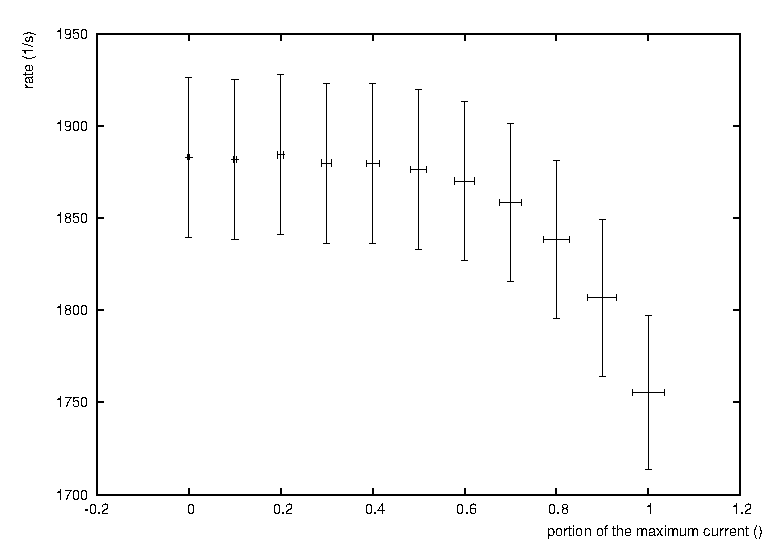
\includegraphics[width = 0.9 \textwidth]{graphics/aircoilCounts/aircoilsCountsCurrent.eps}
  	\caption[Rate dependence on magnetic fields]{Summed rate of all modules over air coil currents. Currents are displayed as parts of the maximum current. A clear decrease in rate is recognizable from \SI{60}{\percent} of the maximum current upwards.}
  	\label{fig:aircoilCountsCurrent}
  \end{figure}
  

  %% ===========================
  \section{Module Stability}
  \label{ch:Analysis:sec:Module Stability}
  %% ===========================  
  If consistent factual statements on muon induced background are to be made, the modules need to work stable over the course of days, as rates are supposed to be comparable. For this reason, over the Christmas time 2012, a two-weekly measurement of half hourly runs was taken, see table \ref{tab:airCoilSettingsChristmas} for air coil settings used. Runs myo00000051 to myo00000675 contain the data of this measurement.
  \begin{table}
  \centering
   \begin{tabular}{|l|ccccccc|c|}
    \hline
    &&&&&&&&\\
    Coil \#	&1	&2	&3	&4	&5	&6	&7	&EMCS h	\\
    Current [A]	&10	&10	&14	&25	&42	&39	&54	&50  	\\
    &&&&&&&&\\
    Coil \# 	&8	&9	&10	&11	&12	&13	&14	&EMCS v	\\
    Current [A]	&54	&21	&36	&30	&21	&20	&56	&15    	\\
    &&&&&&&&\\
    \hline
   \end{tabular}
  \caption[LFCS settings stability measurement]{Runtime settings for air coils as proposed and for the commissioning measurements. These were kept static over the two weeks end 2012/beginning 2013}
  \label{tab:airCoilSettingsChristmas}
  \end{table}
  The time slot was chosen because of the lowly frequented spectrometer hall. The thought was to minimize external impacts on the measurement. During data taking, the LFCS coils were active. They generated magnetic fields in which the PMT tubes had to work throughout the measurement. The LFCS settings are found in \ref{tab:airCoilSettingsChristmas}. For analysis, a simple program to count events in variable time bins was written, creating a count histogram for all the runs in the measurement period. The result can be seen in figure \ref{fig:moduleStability}. A fluctuation of \SI{5}{\percent} of the average value is observable. This is describable by fluctuations in atmospheric density, i.e. pressure $\Delta p$ and temperature $\Delta T$ and in muon production height $\Delta h$. The change in relative intensity is decribed by the following equation.
  \begin{equation}
  	\frac{\Delta I}{I} = - (\alpha_\mu\Delta p + \beta \Delta h -\gamma \Delta T)
  	\label{eq:muonStability}
  \end{equation}
  where $\alpha$ is a barometric coefficient in \SI{0.215}{\percent\per\mmHg}, $\beta$ a decay coefficient in \SI{5}{\percent}/\SI{10e3}{\meter} and $\gamma$ a temperature coefficient in \SI{0.1}{\percent\per\kelvin} \cite{muonIntensity}.
  Looking at weather data from \cite{wetterCom} available on a daily basis, the fluctuations resulting from equation \ref{eq:muonStability} do not fit the data very well. Both highest and lowest value for pressure and temperature were used to calculate daily maxima and minima in intensity. The relative change was projected onto the average rate in figure \ref{fig:moduleStability}. Although the order of magnitude does not differ vastly, even the rate development does not always compare to the ones visible in the data of the stability measurements. Several reasons may contribute to this. It has to be kept in mind that the weather data was obtained from a weather station in Rheinstetten, about \SI{20}{\kilo\meter} south of KIT campus north. Furthermore, the station only records data from the lowest atmospheric layer while muons are generated mostly in the upper layers of the atmosphere. Additionally, and this is probably the largest factor here, the muon production height was not included in the analysis as no data was available for this. As all of the fluctuations are in a window of around $\pm$ \SI{5}{\percent}, the modules are stable enough for the purposes needed.
  \begin{figure}
  \centering
	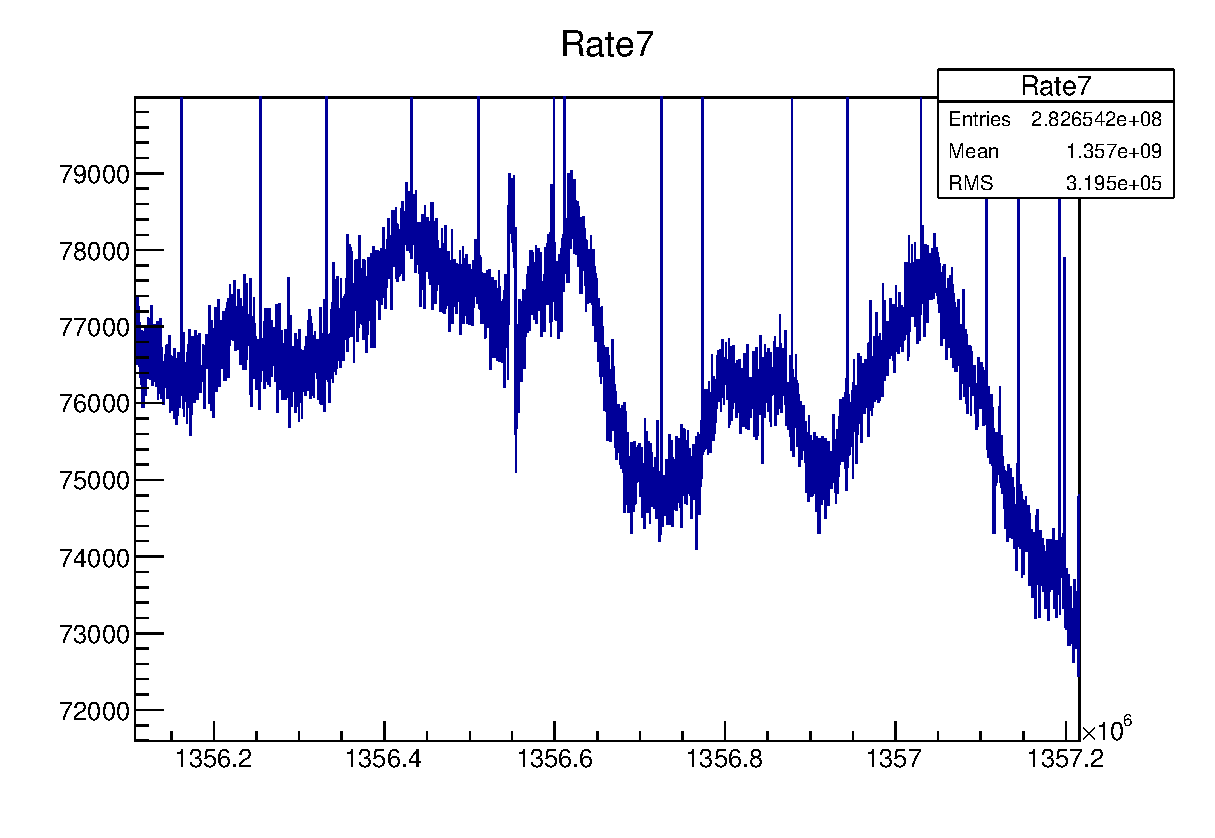
\includegraphics[width = 0.9 \textwidth]{graphics/setup/stability.eps}
  	\caption[Muon module stability]{Counts per five minutes over the course of about two weeks (21-12-2012 to 03-01-2013). The rate deviates \SI{5}{\percent} from the average.}
  \end{figure}

  \begin{figure}
	\centering
  	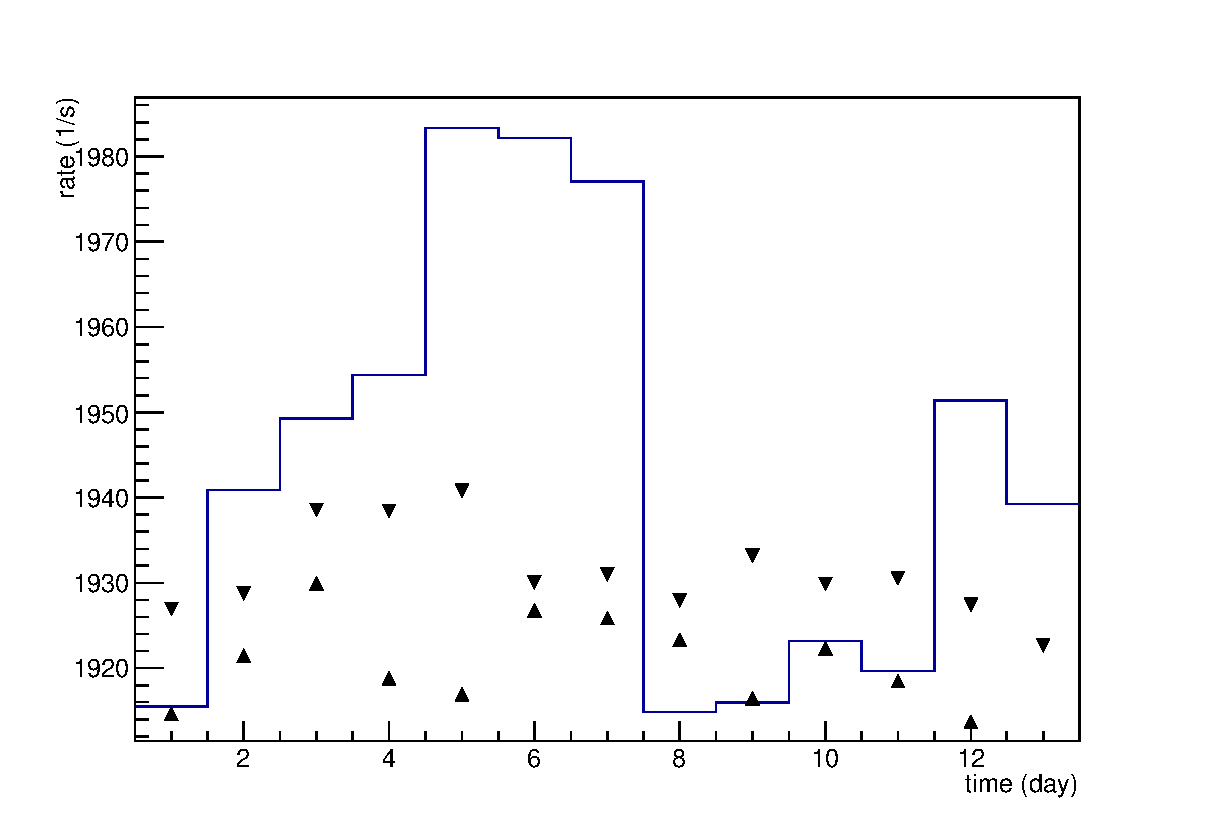
\includegraphics[width = 0.9 \textwidth]{graphics/setup/rateWeather.eps}
  	\caption[Daily average muon rate]{Atmospheric density as a function of time over the course of two weeks the muon measurements took place. Note the }
  	\label{fig:moduleStability}
  \end{figure}

  %% ===========================
  \section{Module Efficiency}
  \label{ch:Analysis:sec:Module Efficiency}
  %% ===========================  
  The runs used for stability measurements, as well as any other run including three modules coaligned in front of each other, can be used to check the middle module for efficiency. For tests on other modules, the geometry would need to be changed so that the one to be checked is in between at least two other modules.
  For analysis, the function determineEfficiency() \ref{ch:Analysis software:sec:methods of the class run:subsec:determineEfficiency}
  has been written.
  The principle is the following: considering the small change in momentum direction high energy muons achieve through interaction with matter, one can assume straight-lined paths. From that follows, that if two parallel planes, that can be used to describe the scintillating volumes, are hit, any other, also parallel plane, in between those two will be hit as well. Keeping this in mind, one can analyse data for events registered in both modules 6 and 8 and cross check whether a event has been detected in module 7 as well. The quota of events in all three modules compared to those detected in 6 and 8 -  including the triple events - shows the efficiency of module 7.
  It shows that during the measurement period end of 2012, the efficiencies were at \todo{rerun} \SI{92.8\pm 3.8 }{\percent} which is less than one would expect at a scintillator thickness of \SI{5}{\centi\meter}.
  For that reason, the filter settings were checked and changed to the boxcar filter with a gap of \SI{150}{\ns} from the before used \todo{exact name} filter. However, the expected efficiency increase was not observable. The average efficiencies were now at \SI{93.4 \pm 3.6}{\percent}, well within the margin of error of the other.
  To examine the problem further modules 3, 4 and 5, that are located next to each other, were used for efficiency measurements as well considering they are stacked in an upright way. Using the program on those three modules resulted in even lower efficiencies of \SI{50\pm 3.2}{\percent}. This raises the question whether this is not an effect of signal filtering, but a previously not considered physics effect. One thing coming to mind is deviation of the muon track from linear forms. This feature would comply with the seemingly lower efficiency at the upright stacked modules, where, at equal bending radii, the ratio of muons traveling around the middle module is higher due to the lower total area in stacking direction.
  This thesis should be tested. This can be done both by simulating the cosmic muons including magnetic fields and empirically by varying the distance between the single modules. The latter is difficult not only because the modules are heavy and not made for lifting (no designated carrying structures), but also because movement always means potential danger to the photomultiplier tubes and their connection to the scintillators.
  Furthermore, if all coils and solenoids were to be turned off simultaneously at some point, one could collect data then and see how efficiencies change during that (there have been runs taken when that was still the case, but only few modules were working properly at that point).
  If the dependence on module distance turns out to be true, but the efficiencies are still below expected values at the lowest possible distances, a possible improvement would be to use pre-amplifiers before signals arrive at the DAQ. These would widen the signals timewise leading to a more easily detectable signal for the filters.
  
  %% ===========================
  \section{Photo Multiplier Tube Test with $^{90}$Sr source}
  \label{ch:Analysis:sec:PhotoMultiplierTests}
  %% ===========================
  
  With sets of four photomultiplier tubes being read out over one cable, and, consequently, via one channel, the test of individual PMTs is not trivial. Nevertheless, a method using a \SI{}{\mega\becquerel} $\rm ^{90}Sr$ source to trigger events was used to check functionality. Of course, all tubes were able to detect the source's $\beta$-electrons at any position but rates were expected to rise as the distance to one of the tubes shrank. A source holder was constructed from acrylic glass to shield the user from radiation and to attach the source to the modules, as a large dependence of rate on the position was found when the source was simply duct taped to the modules. As the foil mantling of the modules absorbs a large part of the radiation emitted from the source, it had to be ensured that the number of layers was equal for all measurements. This was given only below the modules as the foil has been folded around them at the ends in a gift wrapping way. Thus, the source was pretty far away from the photomultiplier tubes making it more difficult to distinguish between them. A first measurement was to check for exactly this distinguishability.


  \begin{figure}
  \centering
   	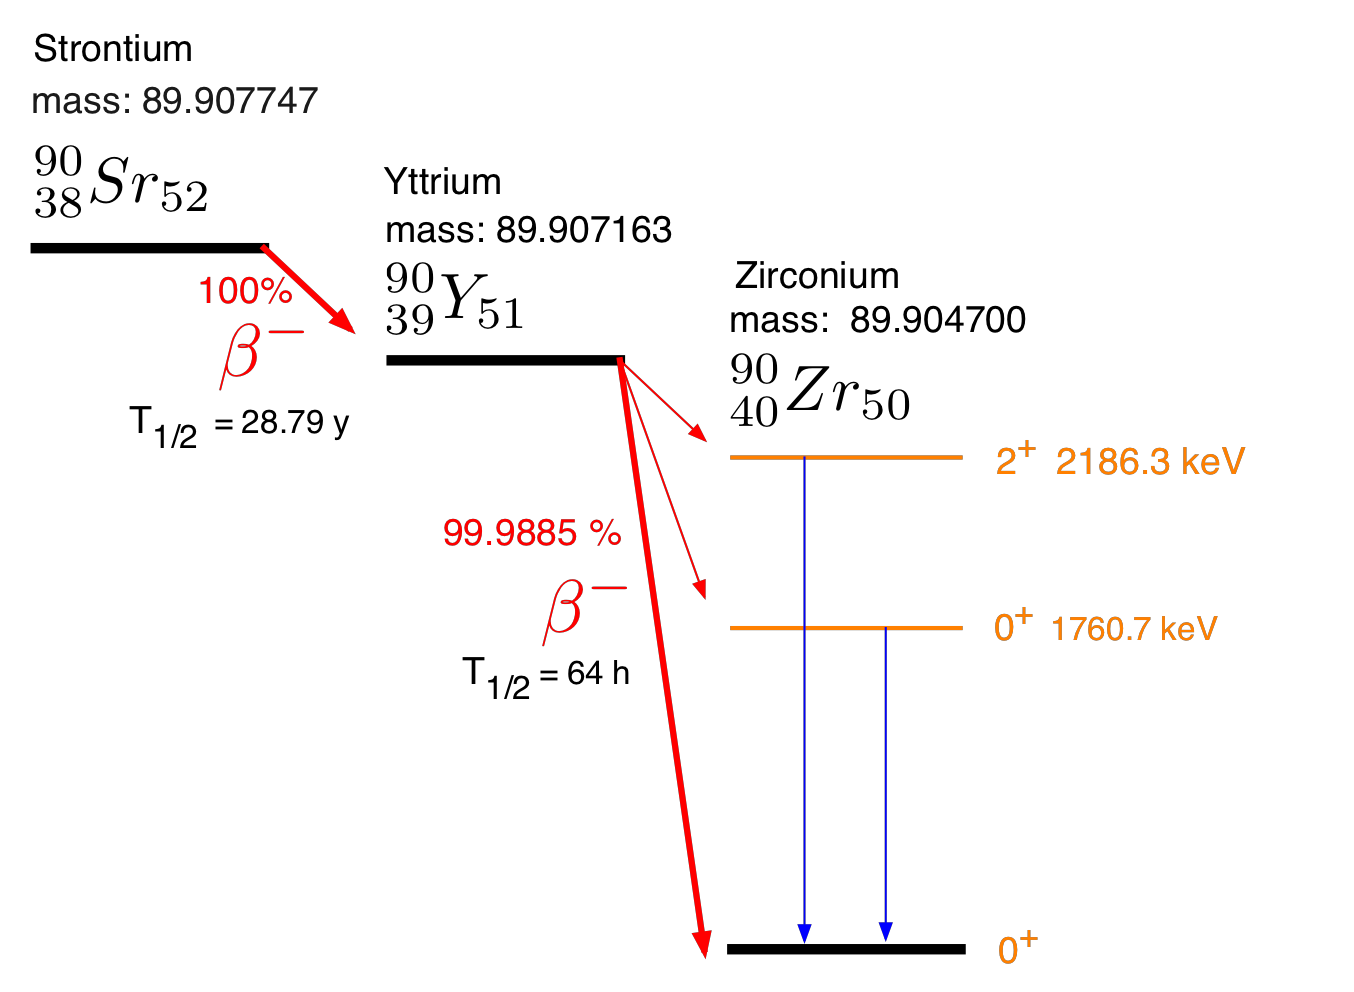
\includegraphics[width = 0.5 \textwidth]{graphics/cobalt/Sr90_decay.eps}
  	\caption[Cobalt decay scheme]{Decay scheme of $^{90}$Sr: first a lower energetic decay to $^{90}$Y emitting \SI{544}{\kilo\electronvolt}/\SI{}{\square c} electrons, from that most probably a higher energetic decay to $^{90}$Zr ground state (\SI{2.29}{\mega\electronvolt}/\SI{}{\square c} electrons) or, with low probabilty, to one of two of its excited states.}
  \end{figure}
  The first though of being able to clearly identify the single PMT positions was soon dropped as all of the PMTs seemed to detect too much of the source's decays at any position (figure \ref{perpendicularScan}).
  This behaviour got worse moving away from the photomultiplier tubes as the distances to the individual tubes equalized. At the same time, the closer the source was moved to the PMT tubes, the larger the position dependence got making it difficult to compare results (figure \ref{} ).
  That is why it was decided to measure at the four points the PMTs were located at and compare both the behavior of the rates and their averall value.
  As one can see a rise in rate at the positions the tubes are located at, it was decided that four measurements per module and side were sufficient, especially as all measurements can afterwards be compared to each other.
  The tube positions at \todo{n,n,n,n cm} were used as measurement positions as well. For each side, a run has been taken containing five minute subruns for every position. Figure \ref{fig:SrRatesPMT12} to \ref{fig:SrRatesPMT678} show the result of these measurements. One can see that the general shapes compare well to the others. Exceptions are modules 2B and 6B that show lower rates than the others. This has been compensated for by a adaption of acceleration voltages.
 
   \begin{figure}
  	\centering 
  	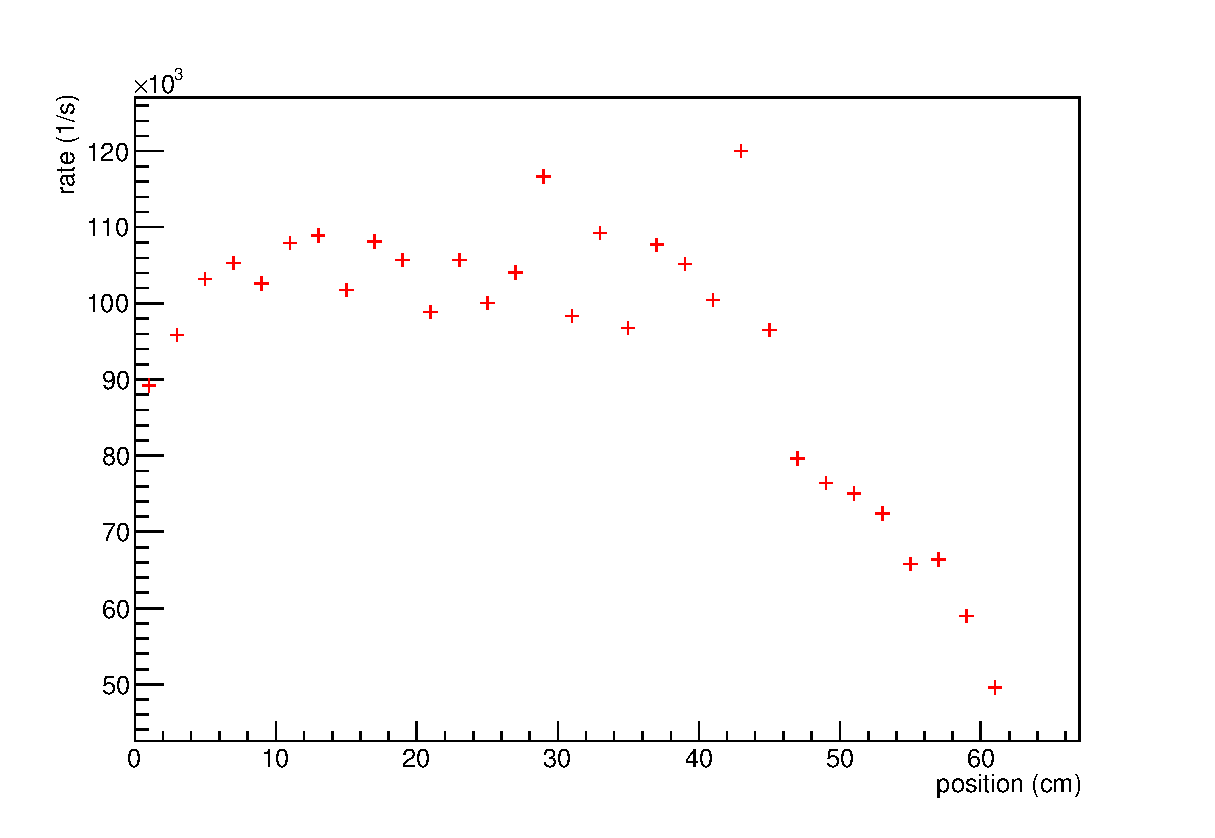
\includegraphics[width = 0.9\textwidth]{graphics/cobaltRate/6parallel.eps}
  	\caption[Cobalt parallel scan]{One of multiple scans taken showing that individual PMT tube positions can not be resolved. The rate at different positions along a line parallel to the PMT alignment is plotted. Only the peripheral areas show drops in rate as the angular coverage of the source gets smaller there.}
  	\label{fig:parallelScan}
  \end{figure}
  
	\begin{figure}
  	\centering 
  	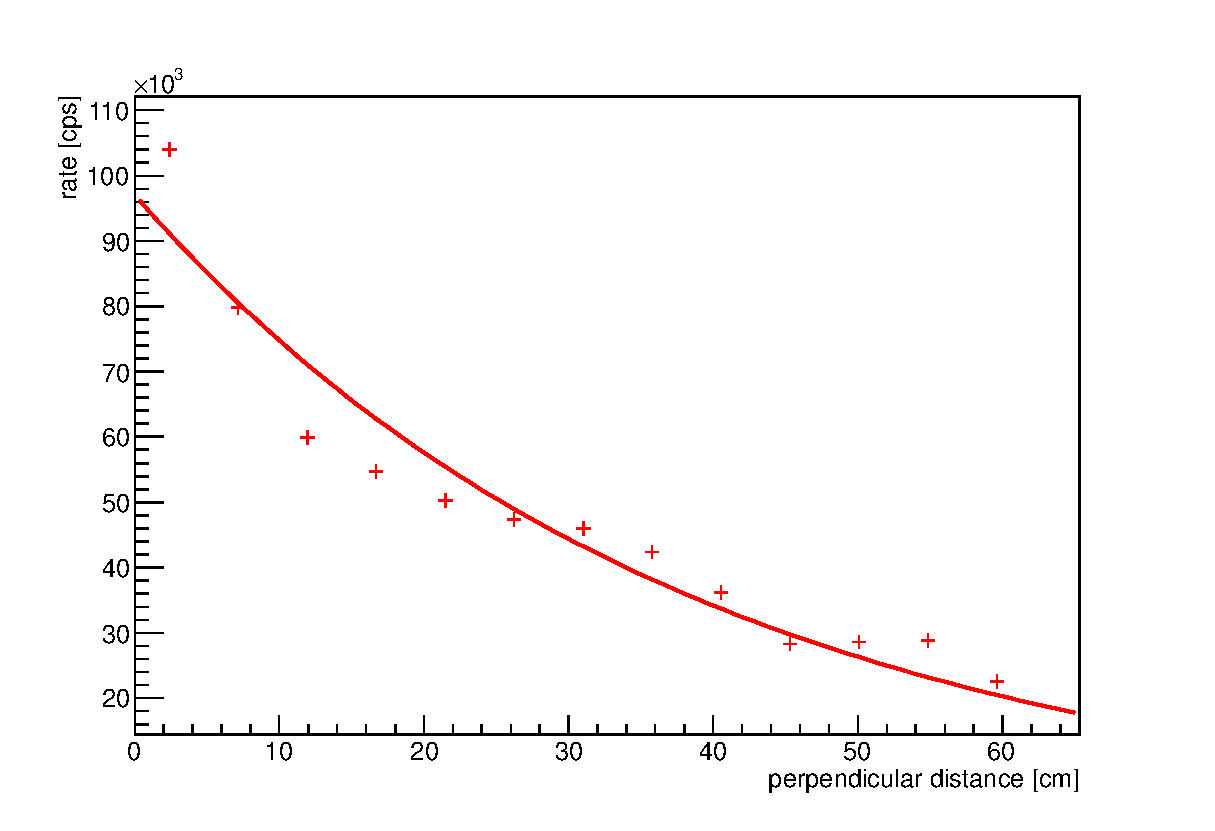
\includegraphics[width = 0.9\textwidth]{graphics/cobaltRate/6perpendicularScan.eps}
  	\caption[Cobalt perpendicular scan]{A position scan along a line perpendicular to the PMT alignment. The rate decreases strongly as the distance gets larger.}
  	\label{fig:perpendicularScan}
  \end{figure}


  
  \begin{figure}
		\centering
		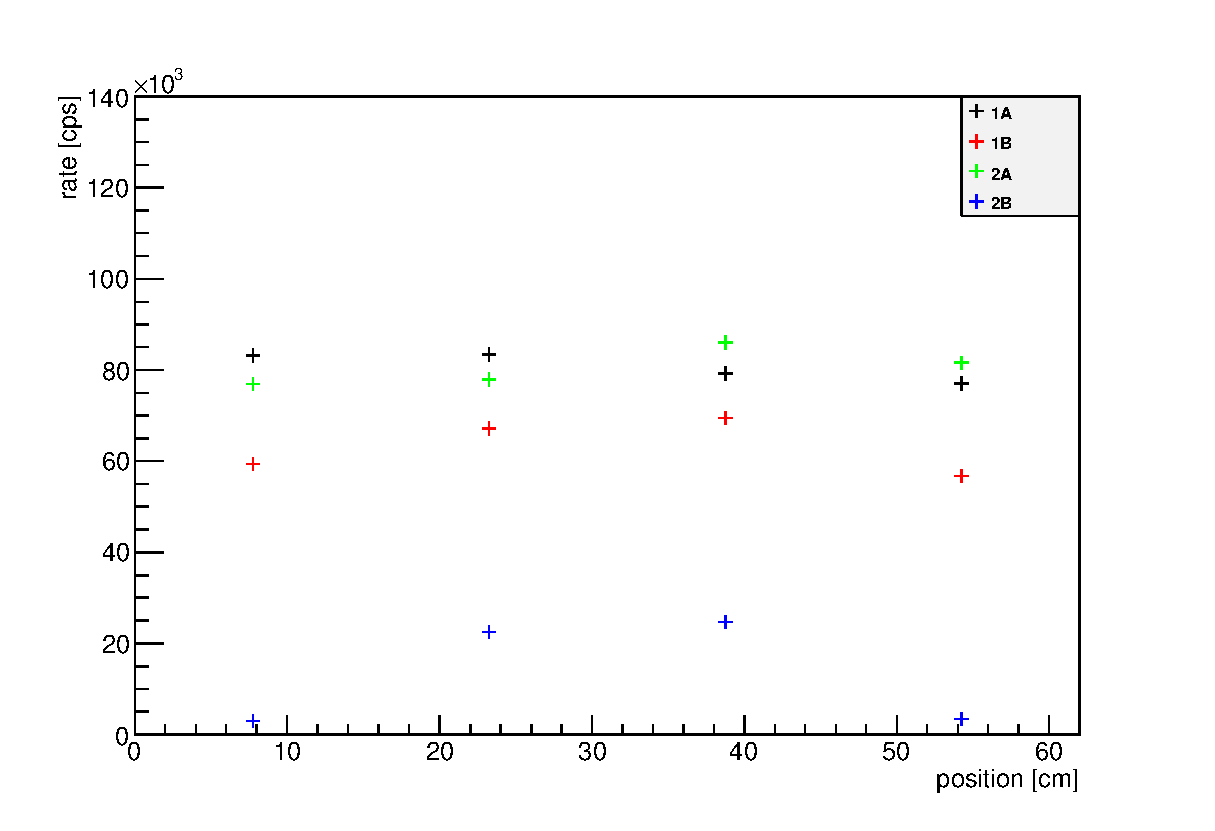
\includegraphics[width = 0.9\textwidth]{graphics/analysis/12final.eps}
  	\caption[Testing of muon modules with Sr source - Modules 1 \& 2]{Measurements with the source at four different positions. Both sides of modules 1 and 2. Noticable are the much lower rates for module 2B which is one of the two that was later set to \SI{1.6}{\kilo\volt} acceleration voltage. }
  	\label{fig:SrRatesPMT12}
  \end{figure}
    \begin{figure}
		\centering
		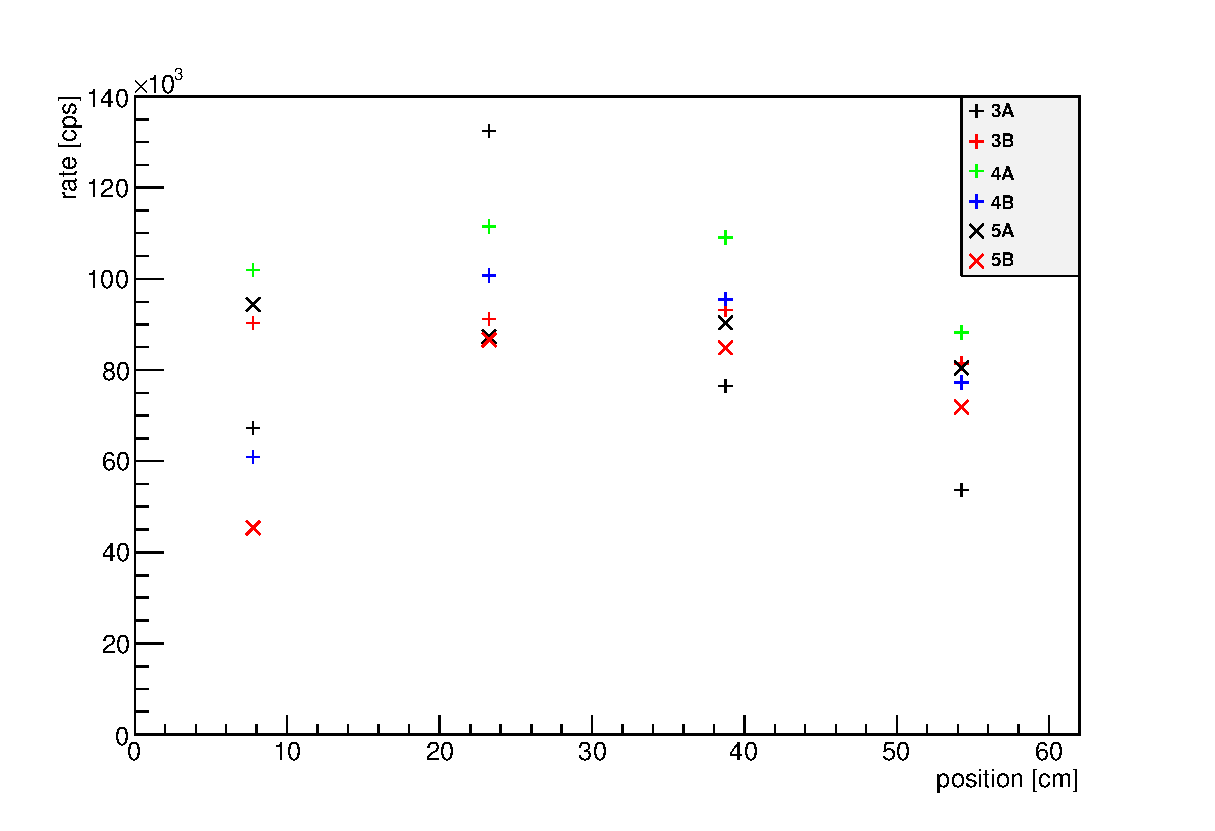
\includegraphics[width = 0.9\textwidth]{graphics/analysis/345final.eps}
  	\caption[Testing of muon modules with Sr source - Modules 3 - 5]{Measurements with the source at four different positions. Both sides of modules 3 to 5 are shown. Except for single measurement points that are standing out, the different sides show similar rates. }
  	\label{fig:SrRatesPMT345}
  \end{figure}
    \begin{figure}
		\centering
		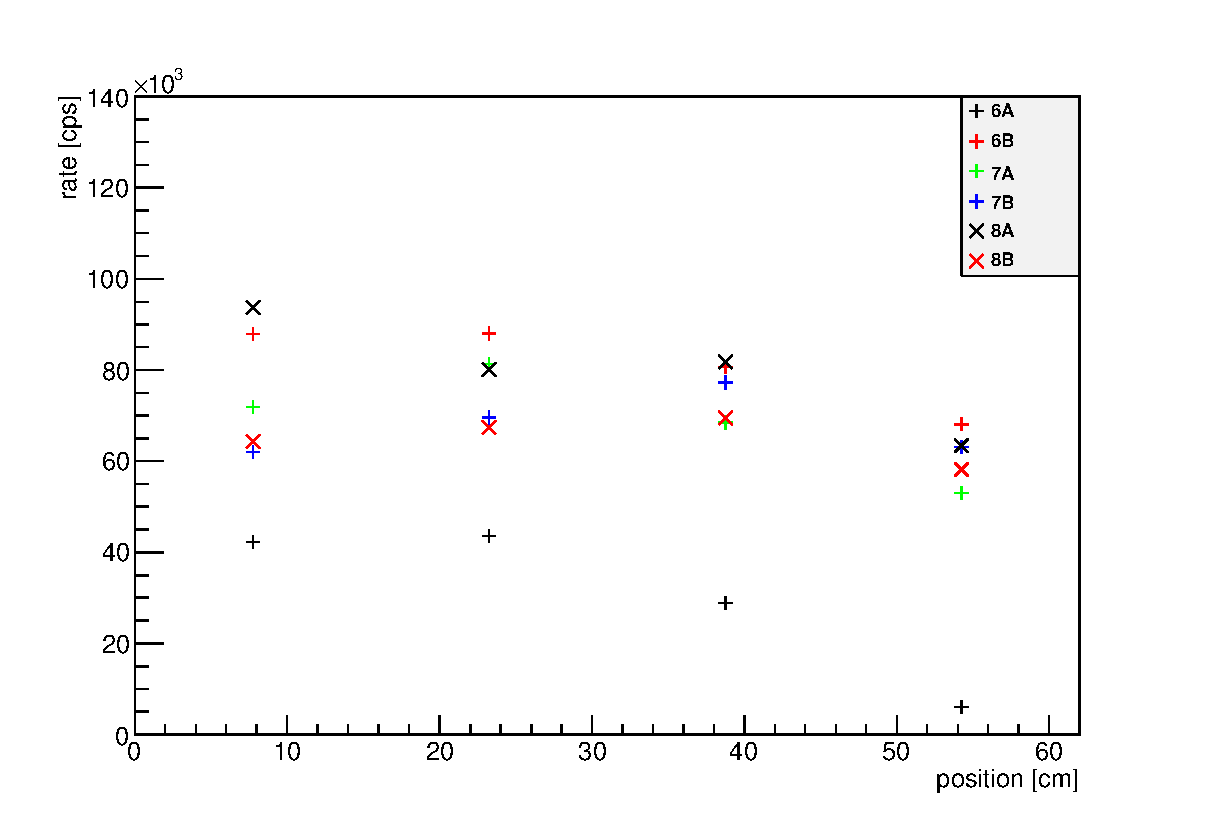
\includegraphics[width = 0.9\textwidth]{graphics/analysis/678final.eps}
  	\caption[Testing of muon modules with Sr source - Modules 6 - 8]{Measurements with the source at four different positions. Both sides of modules 6 to 8. Noticable are the lower rates for module 6B which again is one of the two that was later set to \SI{1.6}{\kilo\volt} acceleration voltage. }
  	\label{fig:SrRatesPMT678}
  \end{figure}

    %% ===========================
  \section{Synchronisation of moun module and FPD DAQs}
  \label{ch:Analysis:sec:Synchronisation of moun module and FPD DAQs}
  %% ===========================  
  Measuring time differences between detector signals and muon events on a \SI{}{\micro\second} scale requires exact synchronization of the two different DAQs. For this purpose, a clock has been designed sending signals at two frequencies: one at \SI{1}{\hertz} and one at \SI{10e6}{\hertz} internally converted to a \SI{20 e 6}{\hertz} signal by the DAQ. Those signals can be synchronized to the timestamps of GPS satellites if a GPS antenna is connected. This has not yet been done as relative synchronization between the two crates is sufficient for the purposes of finding correlations between muon and detector events. As the cable length for signal transmission is pretty extensive - around \SI{50}{\meter} - it was decided to use optical fibers instead of CAT 5 cabling. As two signals need to be transmitted, paired \todo{connection type name} fibers were used. The clock itself has optical outputs, the DAQ though needs converters from optical to electrical signals and a modified SLT back panel card to receive the converted 
  signals via Cat5 cabling.
  To test the setup, the muon DAQ was moved to the detector platform. Both crates were fed by a pulser signal. Runs at different frequencies were recorded to test both the synchronization and the detection of events. To synchronize timestamps to an external signal, the FLT cards drop down menu needs to be set to \todo{look up} and the SLT needs to be set to \todo{lookup too}.
  At first, manually triggered signals were used in minute runs to check the timestamps equality. Several runs were taken, all showing that the events were shifted by several \SI{}{\micro\second}.
  In close cooperation with the IPE it was found that this was merely a problem of firmware versioning as well as software settings in ORCA resolving the problem quickly. After installing the latest firmware, more runs were taken now displaying the desired behavior.
  The spread over the bins makes an estimate of the actual synchronization possible. 
  \begin{figure}
  \centering
  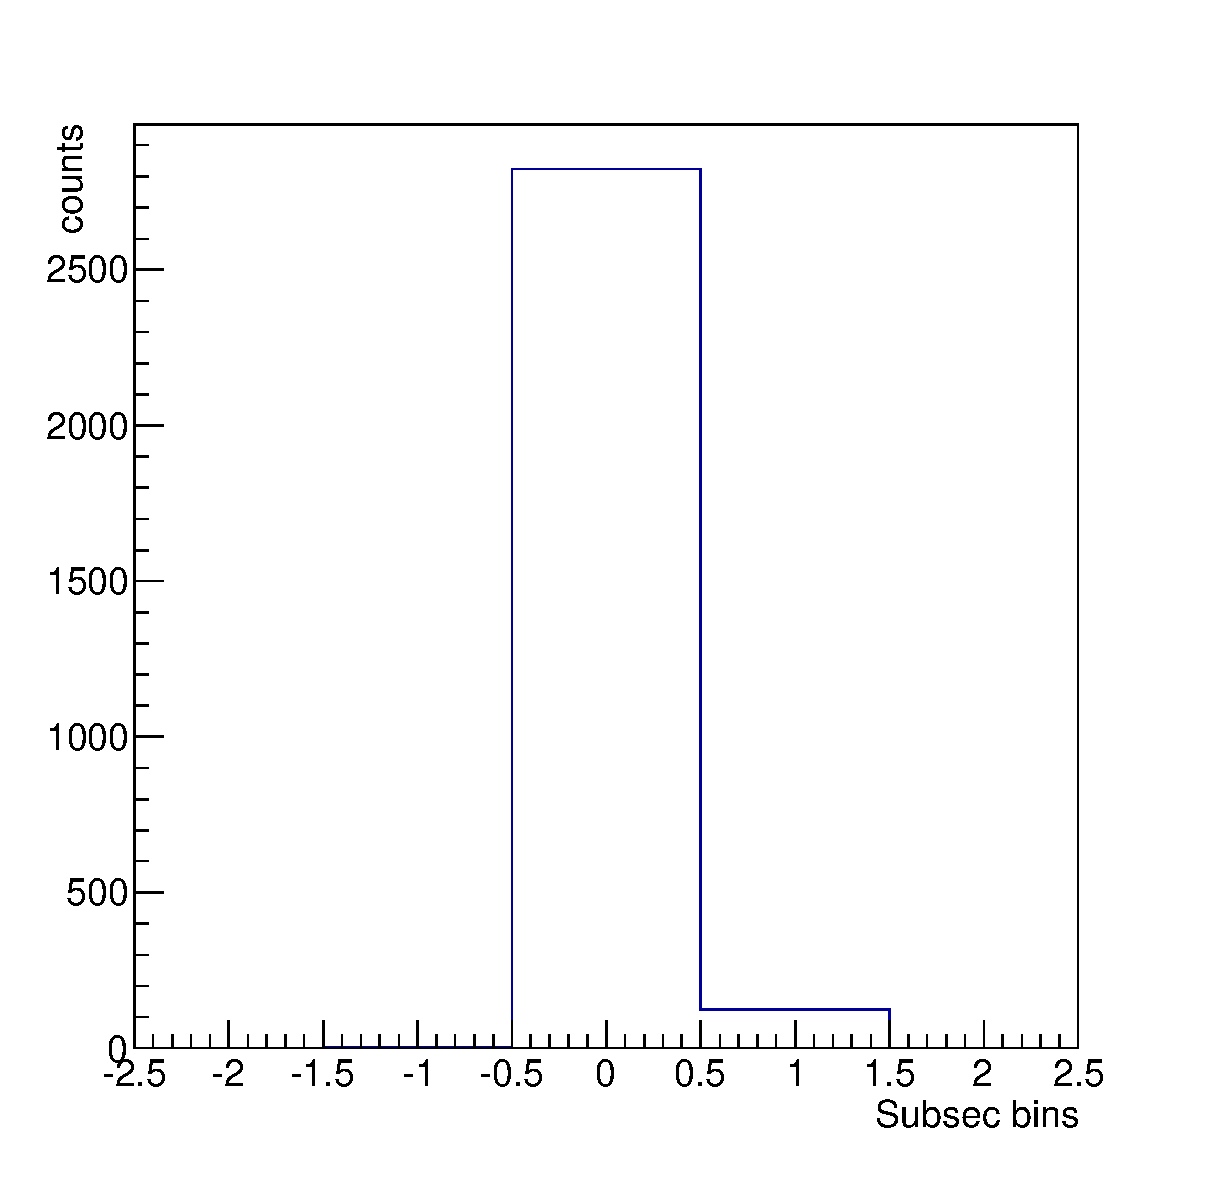
\includegraphics[width = 0.9 \textwidth]{graphics/sync/sync.eps}
	\caption[Synchronisation new firmware]{Time differences between events after firmware upgrades. The difference in subsecond counts, i.e multiples of \SI{50}{\nano\second} is displayed. Differences between the event times are within one bin.}
  \end{figure}
  Following the manually triggered events, runs with fixed frequency events were recorded, raising the frequency to up to \SI{10}{\kilo\hertz}. Doing so, different recording modes and filter settings were applied - see table \ref{tab:syncTests}. All the tests worked fine including starting one DAQ's run way ahead of the other or mixed filter settings. Those events recorded in both run files were always synchronized.
  \begin{table}
  \centering
  	\begin{tabularx}{0.9 \textwidth}{|X|cc|}
  	\hline
  		\bf{Settings} & \bf{fpd run} & \bf{myo run}\\	
  		\hline
  		\multicolumn{3}{|c|}{Pulser voltage 250mV, freq (sampling) 100000, waveform: needle negative}\\
  		\hline
		as before, but 300sec runs & 4174 & 710 \\
		as before, but 300sec runs and energy+trace mode (sync) & 4175 & 711 \\
		5 random pulses within 60sec run & 4176 & 712 \\
		pulser frequency: 1 Hz, 60sec run & 4177 & 713 \\
		pulser frequency: 10 Hz, 60sec run & 4178 & 714 \\
		pulser frequency: 100 Hz, 60sec run & 4180 & 715 \\
		pulser frequency: 1 kHz, 60sec run & 4181 & 716 \\
		pulser frequency: 10 kHz, 60sec run & 4182 & 717 \\
		Pulser:&&\\
		\hline
		\multicolumn{3}{|c|}{Pulser voltage 150mV, Freq (sampling) 1000, waveform: Pin diode negative}\\
		\hline
		5 random pulses within 60sec run & 4184 & 719 \\
		increased thresholds from 500 to 1000 (both)
		pulser frequency: 1 Hz, 60sec run & 4185 & 720 \\
		pulser frequency: 10 Hz, 60sec run & 4186 & 721 \\
		pulser frequency: 10 Hz, 300sec run & 4187 & 722 \\
		pulser frequency: 100 Hz, 300sec run & 4188 & 723 \\
		pulser frequency: 10 Hz, 300sec run & 4189 & 724 \\
		\hline
		\multicolumn{3}{|c|}{ Removing Cat5 cables from synchronization clock and }\\
		\multicolumn{3}{|c|}{ installing fiber optic cables + converter boxes}\\
		
		\hline
		pulser frequency: 0.2 Hz, 60sec run & 4190 & 725 \\
		5 random pulses within 60sec run, both energy mode & 4191 & 726 \\
		pulser frequency: 1 Hz, both energy mode, 60sec run & 4192 & 727 \\
		pulser frequency: 10 Hz, both energy mode, 60sec run & 4193 & 728 \\
		pulser frequency: 10 Hz, both energy mode, 300sec run & 4194 & 729 \\
		pulser frequency: 100 Hz, both energy mode, 300sec run & 4195 & 730 \\
		pulser frequency: 10 Hz, both energy+trace (sync) mode, 300sec run & 4196 & 731 \\
  		\hline
  	\end{tabularx}
	\caption[Synchronization test Settings]{All settings including run numbers tested with the two DAQs from detector system and muon modules. In the leftmost column, pulser settings and run lengths are described. In front of the different parts the pulser settings kept constant for the following measurements are described.}
	\label{tab:syncTests}
  \end{table}

  Afterwards, the muon DAQ was moved back to its original position and the optical fibers were stowed in wire-ways guiding it from the detector platform down to the basement where the muon detection system is located. Another problem occurred here, as signal transmission was impaired by a kink at one of the turns, but was quickly resolved by smooth rewiring.
  Concluding, it can be said that the clock runs continuously without any problems throughout all the measurements - including main spectrometer commissioning measurements.

  
  %% ===========================
  \section{Coincidence Search between Muon- and Detector Events}
  \label{ch:Analysis:sec:Monitor Spectrometer Measurements}
  %% ===========================  
  If one wants to actually detect background induced by muonic events detected by the muon modules, those events need to be correlated to detector events time wise. For this purpose, the analysis code's class run was extended by the member functions TOFHist()\ref{ch:Analysis software:sec:methods of the class run:subsec:TOFHist()} and TOFMuonDet()\ref{ch:Analysis software:sec:methods of the class run:subsec:TOFMuonDet()}, where the former is used for monitor spectrometer analysis and the latter for the main spectrometer. The biggest difference is that, for the main spectrometer, runs by two DAQs leading to different starting times and different lengths are created that need to be compared. Here, the necessity for synchronization from chapter \ref{ch:Analysis:sec:Synchronisation of moun module and FPD DAQs} becomes clear. Different magnetic field configurations were used that can be split into two generalized groups.\\
  Asymmetric magnetic fields are configurations in which the magnetic field lines do not pass through the spectrometer vessel, but are widened to hit the spectrometer wall. This way, muon induced secondary electrons are guided to the detector on cyclotron tracks around those field lines.\\
  In non-axially symmetric configurations, the fieldlines show no rotational symmetry around the z-axis. This change in fields is achieved by an additional coil on top of the monitor spectrometer vessel. At the main spectrometer, it would only be possible using the EMCS coils \ref{ch:The KATRIN experiment:sec:Experimental setup:subsec:Solenoids, LFCS and EMCS system} but no measurements of that kind have been taken until now.
  
  %% =========================
  \subsection{Monitor Spectrometer}
  \label{ch:Analysis:sec:Monitor Spectrometer Measurements:subsec:Monitor Spectrometer}
  %% =========================
  
  Measurements at the monitor spectrometer are easily manageable due to the fast accessibility of all the components and the collection of data in a single run-file through the mini-crate.
  For measurements, high voltage supplies have been added to the \todo{name of the rack} rack and the muon modules were connected to a newly added second FLT-card. Readout was handled by the mini-DAQ , the new FLT card was operated in veto-mode. Gains and thresholds were easily set as only four sides had to be adjusted - compared to the 16 main spectrometer channels. The PMT tubes were operated at \SI{1.5}{\kilo\volt}. The detector gain and threshold settings for the 5 pixel detector have been kept at standard monitor spectrometer operation settings. The detector position though was shifted to the position at which the center pixel exhibited maximum rate and the pairs of east-west and top-bottom pixels showed comparable count rates. Furthermore, the recording mode was switched from histogram-mode to energy-mode as the timestamps for every single event were needed for analysis. 
  Several hourly runs were taken under different magnetic field compositions. Both asymmetric magnetic field (see table \ref{tab:analysis:asymmetricMagneticFields} and non-axially-symmetric field (see table \ref{tab:analysis:nonAxiallySymmetricField} configurations were investigated.
  \begin{table}
	\centering
		\begin{tabular}{c}
		\end{tabular}\\
		\begin{tabular}{|l|l|ccccccc|}
			\hline
			\centering
			
			Measurement &Run &  solenoid &solenoid &inner & outer &outer &emcs x	&emcs y\\
			& 	& source	& detector & aircoil & central aircoil & aircoil& &\\
			\hline
			A & mos00159395& 0&	25&	0&	-4&	-4&	2&	-19.5\\
			\hline
			 B & mos00159396-&&&&&&&\\
			& mos00159398 & 0 & 50& 0 & -8 & -8 & 2 & -19.5\\
			\hline
			C & mos00159399 & 0 & 50& 0 & -7 & -7 & 2 & -19.5\\
			\hline
			D & mos00159400 & 0 & 50& 0 & -6 & -6 & 2 & -19.5\\
			\hline
			E & mos00159401 & 0 & 10& 0 & -2 & -2 & 2 & -19.5\\
			\hline
			F & mos00160713-&&&&&&&\\
			& mos00160717& 0.1 & 12.5 & 0 & -2 & -2 & 0 & 0\\
			\hline
			G & mos00160718-&&&&&&&\\
			& mos00160730 & 0.1 & 12.5 & 0 & -2 & -2 & 0 & 0\\
			\hline
			H &mos00161105-&&&&&&&\\
			& mos00161107 & 0.1 & 12.5 & 0 & -2 & -2 & 0 & 0\\
			\hline
			I &mos00161108-&&&&&&&\\
			 & mos00161110 & 0.1 & 25 & 0 & -2 & -2 & 0 & 0\\
			\hline
		\end{tabular}
		\caption[Asymmetric magnetic field measurements]{Measurements at asymmetric magnetic fields. The source side magnet was turned off for all measurements leaving the flux tube entering the spectrometer walls.}
		\label{tab:analysis:asymmetricMagneticFields}
	\end{table}
	\begin{table}
		\begin{tabularx}{\textwidth}{|L{1.1cm}|>{\centering}X|>{\centering}X>{\centering}X>{\centering}X>{\centering}X>{\centering}X>{\centering}X>{\centering\arraybackslash}X|}
			\hline
			\parbox[t]{2mm}{\multirow{3}{*}{\rotatebox[origin=c]{90}{ Run mos00... }}}
			&\parbox[t]{2mm}{\multirow{3}{*}{\rotatebox[origin=c]{90}{\bf 2 Horizontal loops }}}
			&\parbox[t]{2mm}{\multirow{3}{*}{\rotatebox[origin=c]{90}{solenoid source }}}
			&\parbox[t]{2mm}{\multirow{3}{*}{\rotatebox[origin=c]{90}{solenoid detector }}}
			&\parbox[t]{2mm}{\multirow{3}{*}{\rotatebox[origin=c]{90}{inner aircoil }}}
			&\parbox[t]{2mm}{\multirow{3}{*}{\rotatebox[origin=c]{90}{ outer aircoil }}} 
			&\parbox[t]{2mm}{\multirow{3}{*}{\rotatebox[origin=c]{90}{outer cent. aircoil }}}
			&\parbox[t]{2mm}{\multirow{3}{*}{\rotatebox[origin=c]{90}{EMCS x }}}
			&\parbox[t]{2mm}{\multirow{3}{*}{\rotatebox[origin=c]{90}{EMCS y }}}\\
			
			
			
			&&&&&&&&\\
			&&&&&&&&\\
			&&&&&&&&\\
			&&&&&&&&\\
			&&&&&&&&\\
			&&&&&&&&\\
			&&&&&&&&\\
			\hline
			161111-161125 & 0 & 25 & 25 & 6.8 & -7 & 5 & 0 & -14\\
			\hline
			161126-161129 & +50 & 12.5 & 12.5 & 3.5 & -3.5 & 2.5 & 0 & 0\\
			\hline
			161130-161133 & +25 & 12.5 & 12.5 & 1.75 & -1.75 & 1.25 & 0 & 0\\
			\hline
			161134-161149 & -25 & 12.5 & 12.5 & 1.75 & -1.75 & 1.25 & 0 & 0\\
			\hline
			161150-161155 & -50 & 12.5 & 12.5 & 3.5 & -3.5 & 2.5 & 0 & 0\\
			\hline
			161156-161158 & 0 & 12.5 & 12.5 & 3.5 & -3.5 & 2.5 & 0 & 0\\
			\hline

			
			\hline
		\end{tabularx}
		\caption[Non axially-symmetric magnetic field measurements]{Measurements in energy mode at non axially symmetric magnetic field. Both solenoid and air coil currents have bee changed, though always by a multiplication factor for all of them so that the ration remained the same.}
		\label{tab:analysis:nonAxiallySymmetricField}
		
  	\end{table}
  	
  	
  The TOFHist function (chapter \ref{ch:Analysis software:sec:methods of the class run:subsec:TOFHist()}) has been used to analyze the data as well as ``Beans'' code.
  Both browse through all the muon-events detected and finds any detector event in a definable timespan after (or before) the muon-event. This can be more than one detector-event per muon-event. In all of the settings, a peak is visible at around \SI{2}{\micro\second}. As for count rates, they are a lot higher in the asymmetric magnetic field setup as secondary electrons are guided from their point of origin to the detector instead of mostly being magnetically shielded. In this setup, only the reflection through the rise in magnetic field on the electrons' paths takes its toll on the rate (see section \ref{ch:The KATRIN experiment:sec:MAC-E}).
  As data with a lot of different field configurations was analyzed, the major part of setups and analysis can be found in the annex on pages \pageref{ch:annex:sec:A3}.
  
  
  %% =========================
  \subsection{Main Spectrometer}
  \label{ch:Analysis:sec:Monitor Spectrometer Measurements:subsec:Main Spectrometer}
  %% =========================
  
  Monitor-spectrometer results suggested that the time of flight was well measurable, even if on bigger scale, at the main spectrometer. So, during commissioning measurements, already parallel to first measurements ``M1'', some runs with asymmetric magnetic field have been taken with switched polarity or turned off pre spectrometer magnets compared to standard setup.
  The data was analysed for each single ring of the FPD. Search parameters were the time slot from \SI{0}{\second} to \SI{15}{\micro\second}. Data remained inconclusive at the time (figure \ref{}). 
  The failure to find a clear runtime for electrons induced by muonic events might have been due to the combination of muon module position and the magnetic field setup. In the first measurements, the wall area covered by the flux tubes and the volume surveilled by the muon modules did not overlap very much. Furthermore, due to the very low magnetic field at the wall compared to the volume inside the detector and pinch magnet, most of the induced electrons are magnetically reflected as the maximum polar angle towards magnetic field lines $\theta_{max}$ is defined by
  \begin{equation}
  	\frac{B_{min}}{B_{max}} \approx \frac{\SI{3}{\gauss}}{\SI{4}{\tesla}} = sin^2(\theta_{max})
  \end{equation}
  meaning only angles satisfying the inequation
  \begin{equation}
  	\theta < \arcsin{\sqrt{\frac{B_{min}}{B_{max}}}} = \arcsin{\sqrt{\frac{\SI{3}{\gauss}}{\SI{4}{\tesla}}}} = \SI{0.004}{\degree}
  \end{equation}
	will be able to reach the detector. All others will be reflected and fly back to the wall to be absorbed in the conducting wall material. \todo{set real field values}
	As a result, compared to the monitor spectrometer, where the ratio is a lot greater, less of the muon induced electrons arrive at the detector making long measurements a requirement for good statistics. This leads to detector rates of only around \SI{2}{\cps}, depending on the inner electrode voltages.
	At high inner electrode voltages, the rate increases strongly to \SI{150}{\cps} which is probably due to field emission from the electrodes. Here, the rate of events actually analyzed can be reduced by using energy cuts and excluding pixels with either known problems - for example the two defective pixels - or such covered by the misaligned flapper valve. The energies were cut below \SI{25.6}{\kilo\electronvolt} and above \SI{30.6}{\kilo\electronvolt} including the PAE voltage of \SI{25}{\kilo\volt}\todo{add PAE voltage}.
  
  Analysis for every single pixel was not possible due to far too low statistics, though it might be more conclusive as less different path lengths can contribute to a single pixel. On the other hand, after the non-central alignment of the detector has been fixed using different settings for the LFCS-system, the fields should be rotationally symmetric around the z-axis disregarding small deviations. Assuming this, the path lengths for every pixel of one ring should be very comparable.
  
  
  For better results, different field configurations were used. The first only widened the flux tube so the coverages of the volume surveilled by the muon detectors and the flux tube (figure \ref{fig:mainSpec_B}). The second configuration also densified the field lines in the area of the muon modules. This again raised the probability of seeing electrons from detected muons at the detector, but also raised the angular acceptance by increasing the magnetic field at the walls by a factor of two (figure \ref{mainSpec_9}).
  All in all, three different magnetic field configurations were used, they are shown in figures \ref{fig:mainSpec_100A}, \ref{fig:mainSpec_B}, \ref{fig:mainSpec_9} and described in tables \ref{tab:mainSpecSettings} and \ref{tab:mainSpecRuns} including run numbers.  
  
	
  To raise the overall acceptance of the muon induced events, these measurements were repeated with the main vessel on high voltage of \SI{18.6}{\kilo\volt} accelerating all the electrons towards the FPD.
  Following that presumption, for measurements ``C'' (table \ref{tab:mainSpecRuns}), the setup was changed. The flux tube was returned to its initial setting (figure \ref{fig:mainSpec_100A}) and the muon modules were moved towards the steep cone.
  
  None of the settings showed time peaks as clear as the monitor spectrometer. 
  Simulations of single events show that the fastest particles arrive after times comparable to the ones of the monitor spectrometer, i.e. at \SI{1.5}{\micro\second} (figure \ref{mainSpecSimulation}). This already poses a problem. The anticipated rate of muons through the area of the main spectrometer covered by the flux tube is
  \begin{equation}
  	
  \end{equation}
  which means that the average time between muon events is of equal size as the time of flight for a single electron. 
  
  \begin{figure}
	\centerline{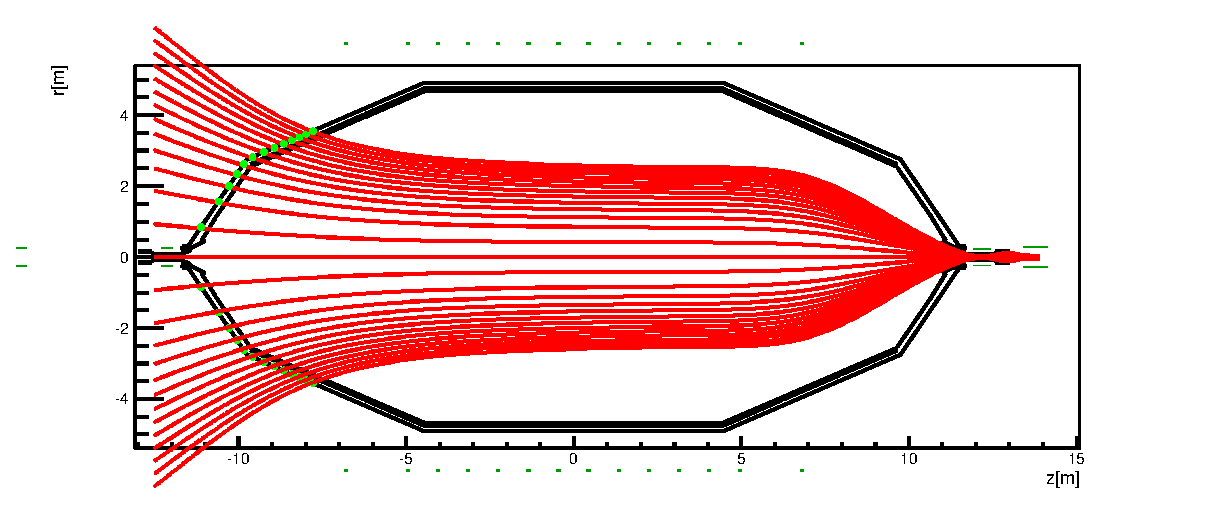
\includegraphics[width = 1.1\textwidth]{graphics/analysis/mainSpec/fieldSimulation/fieldlines_100A.eps}}
	\caption[Flux tube setting A]{First used magnetic field setup. Note that the largest part of the flux tube is in the area of the steep cone. With the initial positions of the muon modules, the probability of the detected muons having caused secondary electrons inside the flux tube was too low.}
  	\label{fig:mainSpec_100A}
  \end{figure}


  \begin{figure}
	\centerline{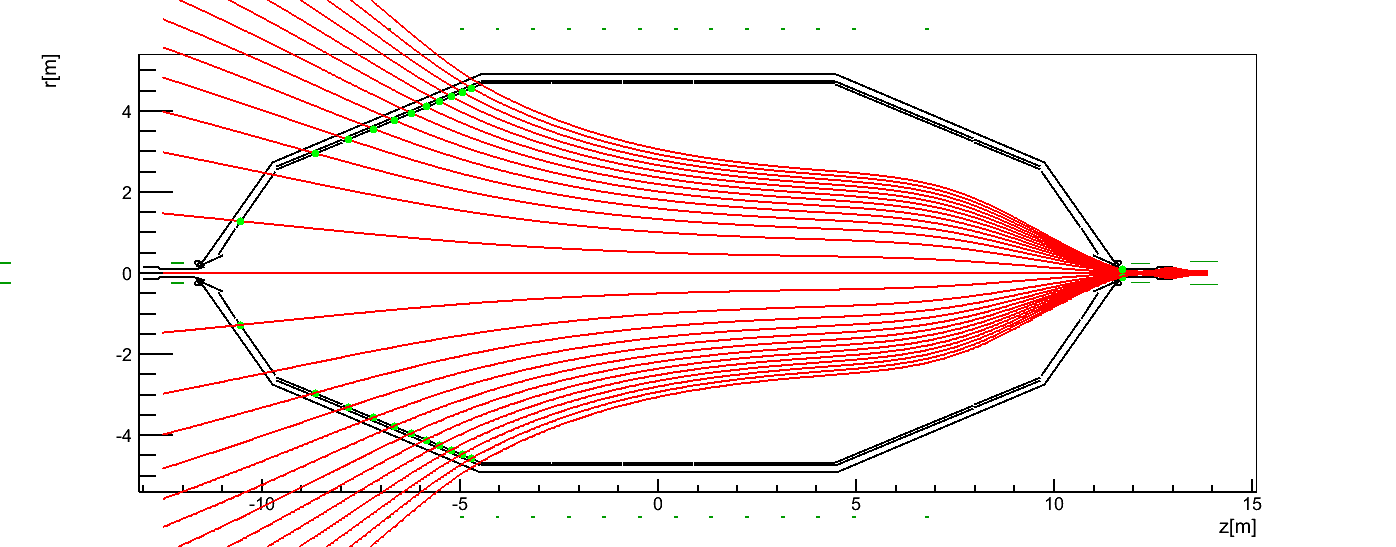
\includegraphics[width = 1.1\textwidth]{graphics/analysis/mainSpec/fieldSimulation/fieldlines.png}}
	\caption[Flux tube setting B]{Widened magnetic flux tube for better coverage by the muon modules. The flat cone is now almost completely covered.}
  	\label{fig:mainSpec_B}
  \end{figure}

  
  \begin{figure}
	\centerline{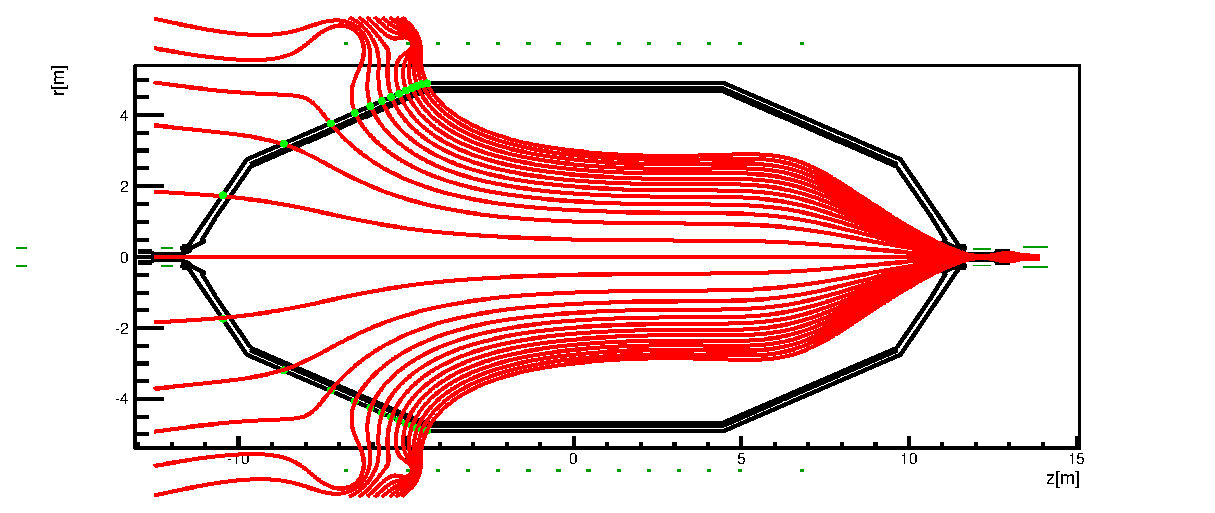
\includegraphics[width = 1.1\textwidth]{graphics//analysis/mainSpec/fieldSimulation/fieldlines_9.eps}}
	\caption[Flux tube setting C]{Flux tube as proposed in \cite{proposalM12}. Here, the LFCS coils on the source side were operated with switched polarity. This creates a denser flux tube in the region of interest.}
  	\label{fig:mainSpec_9}
  \end{figure}

  \begin{figure}
	\centerline{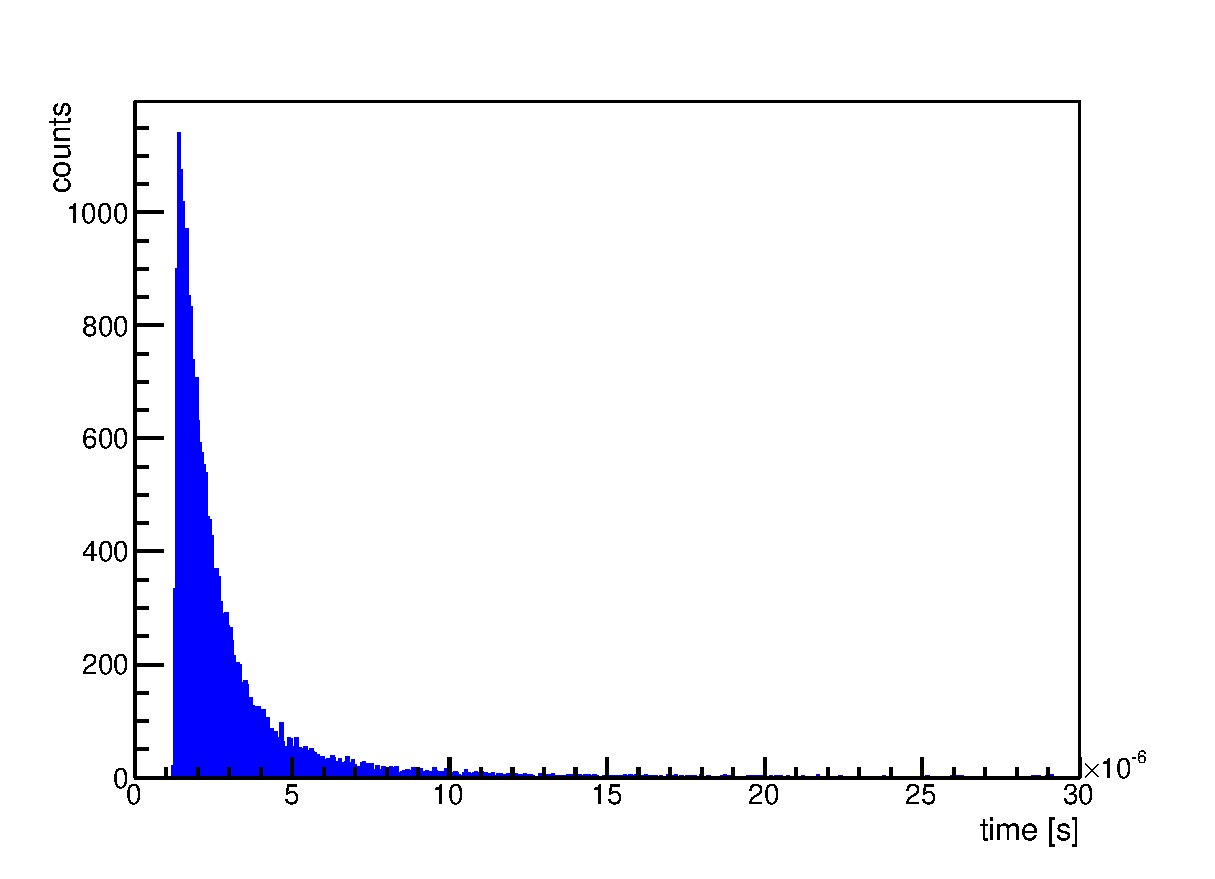
\includegraphics[width = 1.1\textwidth]{graphics/simulation/muonTimeMainSpec.eps}}
	\caption[Main spectrometer simulation]{Time of flight for simulated electrons starting at the spectrometer wall. The ``fastest'' electron arrives at \SI{1.5}{\micro\second}. The distribution has an exponential charakter.}
  	\label{fig:mainSpecSimulation}
  \end{figure}


\begin{table}
	\centering
	\begin{tabular}{|c|cc|cc|}
		\hline
		measurement & myo & & fpd & \\
		setting& start & end & start & end\\
		\hline
		\multirow{2}{*}{A1} & 5159 & 5164 & 939 & 949 \\
		 & 5166 & 5172 & 950 & 977\\
		\hline
		\multirow{1}{*}{B} &5255 & 5256 & 1052 & 1055\\
		\hline
		\multirow{6}{*}{A2}& 6306 & 6307 & 1090 & 1096\\
		& 6308 & 6311 & 1097 & 1104\\
		& 6312 & 6315 & 1105 & 1112\\
		& 6316 & 6321 & 1113 & 1124\\
		& 6322 & 6327 & 1125 & 1136\\
		& 6328 & 6333 & 1137 & 1148\\
		\hline
		
		\multirow{3}{*}{D}& 6401 & 6404 & 1226 & 1229\\
		& 6405 & 6408 & 1230 & 1233\\
		& 6409 & 6412 & 1234 & 1237\\
		\hline
		
		
		
		A3& 7111 & 7134 & 1301 & 1325\\
		\hline
	\end{tabular}
	\caption[Main spectrometer runs]{Main spectrometer runs taken for the search of muon induced background events. The runs are split into groups of same magnetic field settings. The individual settings are listet in \ref{tab:mainSpecSettings}. All group member have different inner electrode voltages, refer to appendix for those as well.}
	\label{tab:mainSpecRuns}
\end{table}

\begin{table}
\centering
	\begin{tabularx}{\textwidth}{|c|c|c|c|c|c|>{\centering\arraybackslash}X|c|c|}
	\hline
% 		\parbox[t]{2mm}{\multirow{1}{*}{\rotatebox[origin=c]{90}{ Measurement setting }}}&
		\begin{sideways} 
			Measurement setting~
		\end{sideways}&
		\begin{sideways}
		IE[V]
		\end{sideways}&
		\begin{sideways}
			PS I [T]
		\end{sideways}&
		\begin{sideways}
			PS II [T]
		\end{sideways}&
		\begin{sideways}
			Pinch [T]
		\end{sideways}&
		\begin{sideways}
			Det [T]
		\end{sideways}&
		\begin{sideways}
			LFCS [A]
		\end{sideways}&
		\begin{sideways}
			EMCS h [A]
		\end{sideways}&
		\begin{sideways}
			EMCS v [A]
		\end{sideways}\\
		\hline

% 		Meas. & IE[V] & PS I [T] & PS II [T] & Pinch [T] & Det [T] & LFCS [A] & EMCS h [A] & EMCS v [A] \\
		{\bf A1, A2, A3} & -700 & 0 & 0 & 5 & 3.5 & \#1 - \#13: \SI{100}{\ampere}; \#14: \SI{0}{\ampere} & 50 & 9 \\
		\hline
		\multirow{2}{*}{\bf B} & \multirow{2}{*}{0} & \multirow{2}{*}{0} & \multirow{2}{*}{0} & \multirow{2}{*}{5} & \multirow{2}{*}{3.5} & \#1 - \#3: \SI{0}{\ampere}; \#4: \SI{50}{\ampere}; \#4 - \#13: \SI{100}{\ampere}; \#4: \SI{0}{\ampere} & \multirow{2}{*}{50} & \multirow{2}{*}{9} \\
		\hline
		\multirow{2}{*}{\bf C} & \multirow{2}{*}{-600} & \multirow{2}{*}{0} & \multirow{2}{*}{0} & \multirow{2}{*}{5} & \multirow{2}{*}{3.5} & \#1 - \#3: \SI{0}{\ampere}; \#4: \SI{50}{\ampere}; \#5 - \#13: \SI{100}{\ampere} \#14: \SI{0}{\ampere} & \multirow{2}{*}{40} & \multirow{2}{*}{9} \\
		\hline
	\end{tabularx}
	\caption[Main spectrometer magnnetic field settings]{Magnetic field settings for the individual groups from table \ref{tab:mainSpecRuns}}
	\label{tab:mainSpecSettings}
\end{table}

  
  
